\documentclass[10pt]{article}
\usepackage[a4paper,top=6mm,bottom=6mm,left=6mm,right=6mm,
            headheight=0pt,headsep=0pt,footskip=0pt]{geometry}
\usepackage[T1]{fontenc}
\usepackage{amsmath}
\usepackage{amssymb}
\usepackage{array}
\usepackage{xcolor}
\usepackage{tikz}
\usetikzlibrary{arrows.meta,decorations.pathreplacing}

% ================================================================
% Probability flashcards.
%
% One card for each skill on the topic list, with a second card where
% a skill splits into different methods. Each card is written once,
% with \flashcard{<skill>}{<question>}{<answer>}, and \printflashcards
% lays them out twenty to a sheet, four across and five down: a page
% of questions followed by a page of answers.
%
% The answer page mirrors the columns, so that when the file is
% printed double-sided, flipping on the long edge, each answer lands
% on the back of its own question. The left and right margins are
% equal so that the cut lines meet on both sides of the paper. Both
% sides of a card carry its number, so a card can still be matched to
% its answer if the printer shifts the back by a millimetre or two.
%
% The answers use the wording of the Maths Revision topic list. A key
% fact from that sheet is set in bold with \key, and each card ends with
% the sheet's "Remember" line for its topic, set in bold purple with
% \remember to match the purple lines on the sheet.
%
% A card whose contents are too tall for it is drawn with a red frame
% and reported in the log as FLASHCARD OVERFLOW.
% ================================================================

\pagestyle{empty}
\setlength{\parindent}{0pt}
\setlength{\parskip}{0pt}
\setlength{\topskip}{0pt}

\newcommand{\fctopic}{Probability}
\newcommand{\fccode}{Prob}

% ----------------------------------------------------------------
% Card layout
% ----------------------------------------------------------------
\newlength{\fcw}\setlength{\fcw}{0.25\textwidth}
\newlength{\fch}\setlength{\fch}{56mm}
\newlength{\fcpad}\setlength{\fcpad}{2mm}
\newlength{\fciw}\setlength{\fciw}{\dimexpr\fcw-2\fcpad\relax}
\newlength{\fcgap}\setlength{\fcgap}{1.2mm}
\newlength{\fcspare}
\newlength{\fcbodytop}
\newsavebox{\fcheadbox}
\newsavebox{\fcbodybox}

% \flashcard{<skill>}{<question>}{<answer>} stores one card.
\newcounter{flashcard}
\newcommand{\flashcard}[3]{%
  \stepcounter{flashcard}%
  \expandafter\gdef\csname fcskill\arabic{flashcard}\endcsname{#1}%
  \expandafter\gdef\csname fcquestion\arabic{flashcard}\endcsname{#2}%
  \expandafter\gdef\csname fcanswer\arabic{flashcard}\endcsname{#3}}

% The idea a pupil must know to answer this type of question.
\newcommand{\key}[1]{{\bfseries\boldmath #1}}
% The quick way to remember the key step, worded as on the revision sheet.
\definecolor{remember}{RGB}{112,48,160}
\newcommand{\remember}[1]{{\color{remember}\bfseries\boldmath Remember: #1}}
% A line of working, centred and in display style. Used in place of \[ \],
% which leaves an empty line above it when it follows a paragraph break.
\newcommand{\working}[1]{\par{\centering$\displaystyle #1$\par}}

\newcommand{\fcquestionstyle}{\normalsize\raggedright\setlength{\parskip}{4pt}}
\newcommand{\fcanswerstyle}{\footnotesize\raggedright\setlength{\parskip}{2pt}}

% The strip across the top of a card: the skill on the front, and the
% card number on both sides.
\newcommand{\fcnumber}[1]{\makebox[10mm][r]{\color{black!55}\fccode\ #1}}
\newcommand{\fchead}[2]{%
  \begin{minipage}{\fciw}
    \scriptsize\color{blue!50!black}%
    \if#2Q\parbox[t]{\dimexpr\fciw-10mm\relax}{\raggedright\bfseries\csname fcskill#1\endcsname}%
    \else\textbf{Answer}\fi
    \hfill\fcnumber{#1}\par
    \vspace{0.6mm}%
    {\color{blue!30}\hrule height 0.4pt}%
  \end{minipage}}

% \fccard{<number>}{Q or A} draws one side of one card. Questions sit in
% the middle of the space under the strip; answers start at the top.
\newcommand{\fccard}[2]{%
  \sbox{\fcheadbox}{\fchead{#1}{#2}}%
  \sbox{\fcbodybox}{\begin{minipage}{\fciw}%
      \if#2Q\fcquestionstyle\csname fcquestion#1\endcsname
      \else\fcanswerstyle\csname fcanswer#1\endcsname\fi
    \end{minipage}}%
  \setlength{\fcbodytop}{\dimexpr\fcpad+\ht\fcheadbox+\dp\fcheadbox+\fcgap\relax}%
  \setlength{\fcspare}{\dimexpr\fch-\fcpad-\fcbodytop-\ht\fcbodybox-\dp\fcbodybox\relax}%
  \ifdim\fcspare<0pt
    \typeout{FLASHCARD OVERFLOW: \fccode\space #1 #2 by \the\dimexpr-\fcspare\relax}%
    \def\fccut{red}%
  \else
    \typeout{FLASHCARD SPACE: \fccode\space #1 #2 has \the\fcspare\space spare}%
    \def\fccut{black!35}%
    \if#2Q\addtolength{\fcbodytop}{0.5\fcspare}\fi
  \fi
  \begin{tikzpicture}
    \useasboundingbox (0,0) rectangle (\fcw,-\fch);
    \draw[line width=0.3pt,color=\fccut] (0,0) rectangle (\fcw,-\fch);
    \node[anchor=north west,inner sep=0pt] at (\fcpad,-\fcpad) {\usebox{\fcheadbox}};
    \node[anchor=north west,inner sep=0pt] at (\fcpad,-\fcbodytop) {\usebox{\fcbodybox}};
  \end{tikzpicture}}

\newcommand{\fctitle}[2]{%
  \hbox to \textwidth{\footnotesize\vrule width 0pt height 2.6mm depth 0.9mm
    {\color{blue!50!black}\bfseries\fctopic\ flashcards}\quad
    {\color{black!60}Sheet #1 of \fcsheets: \if#2Q questions\else answers\fi}\hfil
    {\color{black!60}Print double-sided, flipping on the long edge.}}%
  \vspace{1mm}}

% \fcpage{<sheet>}{Q or A}. On the answer page the columns run right to
% left, so that each answer is printed on the back of its question.
\newcommand{\fcpage}[2]{%
  \fctitle{#1}{#2}%
  \foreach \fcrow in {1,...,5}{%
    \nointerlineskip
    \hbox{\foreach \fccol in {1,...,4}{%
      \edef\fcn{\the\numexpr(#1-1)*20+(\fcrow-1)*4+\if#2Q\fccol\else(5-\fccol)\fi\relax}%
      \ifnum\fcn>\value{flashcard}%
        \hbox to \fcw{\vrule width 0pt height \fch\hfil}%
      \else
        \fccard{\fcn}{#2}%
      \fi}}}%
  \newpage}

\newcommand{\printflashcards}{%
  \pgfmathtruncatemacro{\fcsheets}{(\the\value{flashcard}+19)/20}%
  \foreach \fcsheet in {1,...,\fcsheets}{\fcpage{\fcsheet}{Q}\fcpage{\fcsheet}{A}}}

% ----------------------------------------------------------------
% Diagrams
% ----------------------------------------------------------------
% \venn{<left set>}{<right set>}{<left only>}{<both>}{<right only>}{<outside>}
% Two overlapping sets inside a universal set. The last argument is
% drawn as it stands, so that it can place the outside region's
% contents anywhere around the circles.
\newcommand{\venn}[6]{%
  \begin{tikzpicture}[x=1mm,y=1mm,font=\scriptsize]
    \draw (0,0) rectangle (44,20);
    \node[anchor=north west,inner sep=1.5pt] at (0,20) {$\xi$};
    \draw (15.5,10) circle (9);
    \draw (28.5,10) circle (9);
    \node at (6,17.5) {$#1$};
    \node at (38,17.5) {$#2$};
    \node[align=center] at (12.5,10) {#3};
    \node[align=center] at (22,10) {#4};
    \node[align=center] at (31.5,10) {#5};
    #6
  \end{tikzpicture}}

% \freqtree{<total>}{<upper group>}{<number>}{<lower group>}{<number>}{<leaf>}{<leaf>}{<leaf>}{<leaf>}
% A frequency tree drawn left to right. The two outcomes on the right
% hand branches are named by \fcleafa and \fcleafb, set before the tree.
\newcommand{\fcleafa}{}
\newcommand{\fcleafb}{}
\newcommand{\freqtree}[9]{%
  \begin{tikzpicture}[x=1mm,y=1mm,font=\scriptsize,
      box/.style={draw,minimum width=7mm,minimum height=3.5mm,inner sep=1pt},
      lab/.style={font=\tiny,inner sep=1pt}]
    \node[box] (r) at (0,0) {#1};
    \node[box] (u) at (14,6.6) {#3};
    \node[lab,above] at (u.north) {#2};
    \node[box] (d) at (14,-6.6) {#5};
    \node[lab,below] at (d.south) {#4};
    \node[box] (uu) at (28,9.3) {#6};
    \node[box] (ud) at (28,3.9) {#7};
    \node[box] (du) at (28,-3.9) {#8};
    \node[box] (dd) at (28,-9.3) {#9};
    \foreach \n in {uu,du}{\node[lab,right] at (\n.east) {\fcleafa};}
    \foreach \n in {ud,dd}{\node[lab,right] at (\n.east) {\fcleafb};}
    \draw (r.east) -- (u.west) (r.east) -- (d.west);
    \draw (u.east) -- (uu.west) (u.east) -- (ud.west);
    \draw (d.east) -- (du.west) (d.east) -- (dd.west);
  \end{tikzpicture}}

\begin{document}

% ================================================================
% Probabilities from equally likely outcomes
% ================================================================
\flashcard{Writing probabilities as fractions, decimals and percentages}
{A bag holds 3 red, 5 blue and 12 green counters. One counter is taken at random.

(a) Find P(red) as a fraction, a decimal and a percentage.

(b) Find P(not red).}
{\key{Probability $=$ number of ways it can happen $\div$ total number of possible outcomes}

$3+5+12=20$ counters
\working{\text{P(red)}=\frac3{20}=0.15=15\%}

\key{Probability it does not happen $=1-$ probability it does happen}
\working{\text{P(not red)}=1-\frac3{20}=\frac{17}{20}}

\remember{Always between 0 and 1: 0 is impossible, 1 is certain.}}

\flashcard{Listing outcomes systematically}
{A caf\'e sells three sandwiches: cheese (C), ham (H) and tuna (T). It sells two drinks: juice (J) and water (W).

List all the meals of one sandwich and one drink.}
{\begin{tabular}{@{}lll}
  C\,J & C\,W & (cheese first)\\
  H\,J & H\,W & (ham first)\\
  T\,J & T\,W & (tuna first)
\end{tabular}

$3\times2=6$ meals (this checks that none are missing)

\remember{Fix one, change the other, work in order, systematically.}}

\flashcard{Sample space diagrams}
{Spinner A is numbered 1, 2, 3. Spinner B is numbered 1, 2, 3, 4. Both spinners are spun and the scores are added.

Find the probability that the total is 5.}
{{\centering
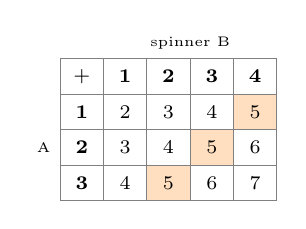
\begin{tikzpicture}[x=5.5mm,y=4.5mm,font=\scriptsize]
  \foreach \a/\b in {1/4,2/3,3/2}{\fill[orange!25] (\b,-\a) rectangle ++(1,1);}
  \draw[step=1,black!50] (0,-3) grid (5,1);
  \node at (0.5,0.5) {$+$};
  \node[font=\tiny,above] at (3,1) {spinner B};
  \node[font=\tiny,left] at (0,-1.5) {A};
  \foreach \b in {1,...,4}{\node at (\b+0.5,0.5) {\textbf{\b}};}
  \foreach \a in {1,...,3}{
    \node at (0.5,-\a+0.5) {\textbf{\a}};
    \foreach \b in {1,...,4}{\pgfmathtruncatemacro{\s}{\a+\b}\node at (\b+0.5,-\a+0.5) {\s};}}
\end{tikzpicture}\par}

All $3\times4=12$ outcomes; 3 of them total 5:
\working{\text{P(total is 5)}=\frac3{12}=\frac14}

\remember{Fix one, change the other, work in order, systematically.}}

\flashcard{Expected results}
{The probability that a spinner lands on red is 0.35. The spinner is spun 200 times.

(a) How many times would you expect it to land on red?

(b) Will it land on red exactly this many times?}
{\key{Expected frequency $=$ probability $\times$ number of trials}
\working{0.35\times200=70}
(a) 70 times

(b) Not necessarily: each spin is random, so 70 is an estimate, not a certainty.

\remember{Probability times the number of goes.}}

\flashcard{Experimental probability}
{A dice is rolled 50 times.

{\centering\footnotesize\setlength{\tabcolsep}{3pt}%
\begin{tabular}{|l|c|c|c|c|c|c|}
  \hline
  Score     & 1 & 2 & 3 & 4 & 5 & 6\\ \hline
  Frequency & 6 & 8 & 7 & 9 & 5 & 15\\ \hline
\end{tabular}\par}

(a) Find the relative frequency of a 6.

(b) Is the dice fair? Explain.}
{\key{Relative frequency $=$ number of times it happened $\div$ total number of trials}
\working{\text{(a)}\quad\frac{15}{50}=0.3}
(b) A fair dice has P(6) $=\frac16\approx0.17$, about 8 sixes in 50 rolls. 15 sixes is far more than this, so the dice may be biased. More rolls would make us more sure.

\remember{More trials, more trust.}}

% ================================================================
% Frequency trees
% ================================================================
\flashcard{Completing a frequency tree}
{\small 60 pupils were asked whether they have a pet. 35 of them are boys. 20 of the boys have a pet. 12 of the girls have a pet.

Complete the frequency tree.

{\centering\def\fcleafa{Pet}\def\fcleafb{No pet}%
\freqtree{60}{Boys}{}{Girls}{}{}{}{}{}\par}}
{{\centering\def\fcleafa{Pet}\def\fcleafb{No pet}%
\freqtree{60}{Boys}{35}{Girls}{\textbf{25}}{20}{\textbf{15}}{12}{\textbf{13}}\par}

Girls: $60-35=25$\\
Boys with no pet: $35-20=15$\\
Girls with no pet: $25-12=13$

\remember{Branches add back up to the number before.}}

\flashcard{Probabilities from a frequency tree}
{\small 80 pupils took a test. One pupil is chosen at random.

{\centering\def\fcleafa{Pass}\def\fcleafb{Fail}%
\freqtree{80}{Revised}{50}{Did not revise}{30}{35}{15}{12}{18}\par}

(a) Find P(pass).

(b) Find P(pass), given that the pupil revised.}
{(a) $35+12=47$ passed, out of 80:
\working{\text{P(pass)}=\frac{47}{80}}
(b) Given they revised: only look at the 50 pupils who revised. 35 of them passed:
\working{\text{P(pass)}=\frac{35}{50}=\frac7{10}}

\remember{`Given' shrinks your total to just that group.}}

% ================================================================
% Venn diagrams
% ================================================================
\flashcard{Completing a Venn diagram}
{In a class of 30 pupils, 17 play football, 13 play tennis, and 5 play both.

Draw a Venn diagram. Find the probability that a pupil chosen at random plays neither sport.}
{{\centering\venn{F}{T}{12}{5}{8}{\node at (40.5,2.5) {5};}\par}

Overlap 5, football only $17-5=12$, tennis only $13-5=8$, outside $30-12-5-8=5$
\working{\text{P(neither)}=\frac5{30}=\frac16}

\remember{Fill the overlap first, then the rest, then outside.}}

\flashcard{Venn diagram notation}
{\small A number from 1 to 12 is chosen at random. A is the multiples of 2 and B is the multiples of 3.

{\centering\venn{A}{B}{2\quad4\\[2pt]8\quad10}{6\\[2pt]12}{3\\[2pt]9}%
  {\node at (3,10) {1}; \node at (41,10) {5}; \node at (3,2.5) {7}; \node at (41,2.5) {11};}\par}

Find P$(A\cap B)$, P$(A\cup B)$ and P$(A')$.}
{\key{$A\cap B$ (A and B) is the overlap.\\
$A\cup B$ (A or B or both) is inside the circles.\\
$A'$ (not A) is outside circle A.}

$A\cap B$ is 6, 12:
\working{\text{P}(A\cap B)=\frac2{12}=\frac16}
$A\cup B$ is 2, 3, 4, 6, 8, 9, 10, 12:
\working{\text{P}(A\cup B)=\frac8{12}=\frac23}
$A'$ is 1, 3, 5, 7, 9, 11:
\working{\text{P}(A')=\frac6{12}=\frac12}}

\flashcard{Conditional probability}
{\small 40 people were asked whether they own a cat (C) or a dog (D).

{\centering\venn{C}{D}{9}{6}{15}{\node at (40.5,2.5) {10};}\par}

A dog owner is chosen at random. Find the probability that they also own a cat.}
{Given they own a dog: only look inside the dog circle.
\working{\text{P(cat)}=\frac6{6+15}=\frac6{21}=\frac27}
($\frac6{40}$ is P(cat and dog), which is a different question)

\remember{`Given' shrinks your total to just that group.}}

\printflashcards

\end{document}
